\section{Risorse}
\subsection{Grafo di Holt Generale (classi e processi)}
\begin{center}
	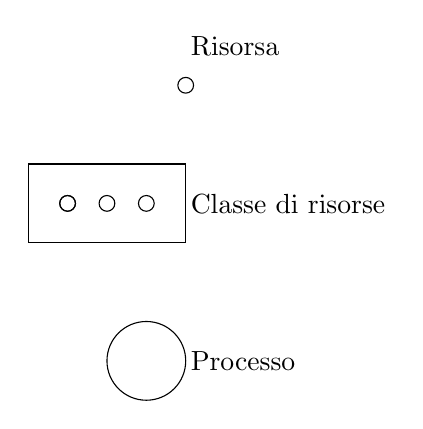
\begin{tikzpicture}
		\draw[draw=black, thin, solid] (-2.00,3.00) circle (0.1);
		\draw[draw=black, thin, solid] (-2.50,-0.50) ellipse (0.50 and 0.50);
		\draw[draw=black, thin, solid] (-4.00,2.00) rectangle (-2.00,1.00);
		\draw[draw=black, thin, solid] (-3.50,1.50) circle (0.1);
		\draw[draw=black, thin, solid] (-3.50,1.50) circle (0.1);
		\draw[draw=black, thin, solid] (-3.00,1.50) circle (0.1);
		\draw[draw=black, thin, solid] (-2.50,1.50) circle (0.1);
		\node[black, anchor=south west] at (-2.06,3.25) {Risorsa};
		\node[black, anchor=south west] at (-2.06,1.25) {Classe di risorse};
		\node[black, anchor=south west] at (-2.06,-0.75) {Processo};
	\end{tikzpicture}
\end{center}
Per gli archi si può segnare la molteplicità, e nelle classi il numero di risorse non assegnate.

\subsection{Detaction and recoverty - Caaso 1}
Teorema: Siano le risorse ad'accesso mutualmente esclusivo, seriali e non prerilasciabili. Con una risorsa per classe si ha deadlock$\iff$ Holt contiene un ciclo (attesa circolare).

Dimostrazione: In un grafo di Holt si ha attesa circolare se si ha attesa circolare nella rispettiva variante di grafo Wait-For (elimina le risorse collassando gl'archi appropriati).

\begin{center}
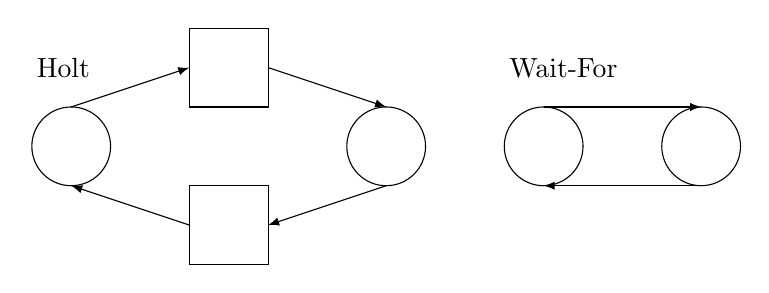
\begin{tikzpicture}
	\draw[draw=black, thin, solid] (-4.00,1.00) rectangle (-3.00,0.00);
	\draw[draw=black, thin, solid] (-4.00,3.00) rectangle (-3.00,2.00);
	\draw[draw=black, thin, solid] (-1.50,1.50) ellipse (0.50 and 0.50);
	\draw[draw=black, thin, solid] (0.50,1.50) ellipse (0.50 and 0.50);
	\draw[draw=black, thin, solid] (2.50,1.50) ellipse (0.50 and 0.50);
	\draw[draw=black, -latex, thin, solid] (-3.00,2.50) -- (-1.50,2.00);
	\draw[draw=black, -latex, thin, solid] (-1.50,1.00) -- (-3.00,0.50);
	\draw[draw=black, -latex, thin, solid] (-4.00,0.50) -- (-5.50,1.00);
	\draw[draw=black, -latex, thin, solid] (0.50,2.00) -- (2.50,2.00);
	\draw[draw=black, -latex, thin, solid] (2.50,1.00) -- (0.50,1.00);
	\draw[draw=black, thin, solid] (-5.50,1.50) ellipse (0.50 and 0.50);
	\draw[draw=black, -latex, thin, solid] (-5.50,2.00) -- (-4.00,2.50);
	\node[black, anchor=south west] at (-6.06,2.25) {Holt};
	\node[black, anchor=south west] at (-0.06,2.25) {Wait-For};
\end{tikzpicture}
\end{center}

\subsection{Detaction and recoverty - Caaso 2}
Teorema: Siano le risorse ad'accesso mutualmente esclusivo, seriali e non prerilasciabili. Con più risorse per classe si ha deadlock $\iff$ Holt non è completamente riducibile (eliminazione tutti archi).

\subsection{Detaction and recoverty - Knot}
Teorema: Siano le risorse ad'accesso mutualmente esclusivo, seriali e non prerilasciabili. Con una richiesta sospespa per processo si ha deadlock $\iff$ esiste un knot.

\subsection{Stato SAFE - algoritmo del banchiere}
Sia $s$ una permutazione dei valori $1,\dots,N$ e $s(i)$ l'i-esima posizione nella sequenza. Si calcola il vettore \textbf{avail} cosi:
\begin{enumerate}
	\item avail[1]=SC
	\item avail[1+j]=avail[j]+$p_{s(j)}$, con i=$1,\dots,N-1$
\end{enumerate}
Uno stato del sistema è safe se vale: $n_{s(j)}$<=avail[j], con j=1,$\dots$,N.

Con il banchiere a singola valuta basta ordinare in modo crescente gli $n_i$ per assicurare lo stato SAFE.

Nel caso multi valuta si aggiunge il pedice k della valuta.

Con il banchiere multi valuta ogni vlauta ha un suo ordine.